\documentclass[11pt]{beamer}
\usetheme{default}

% acronyms for text or math mode
\newcommand {\ccast} {\mbox{\small CCAST}}
\newcommand {\cris} {\mbox{\small CrIS}}

\newcommand {\airs} {\mbox{\small AIRS}}
\newcommand {\iasi} {\mbox{\small IASI}}
\newcommand {\idps} {\mbox{\small IDPS}}
\newcommand {\nasa} {\mbox{\small NASA}}
\newcommand {\noaa} {\mbox{\small NOAA}}
\newcommand {\nstar} {\mbox{\small STAR}}
\newcommand {\umbc} {\mbox{\small UMBC}}
\newcommand {\uw}   {\mbox{\small UW}}

\newcommand {\fft}  {\mbox{\small FFT}}
\newcommand {\ifft} {\mbox{\small IFFT}}
\newcommand {\fir}  {\mbox{\small FIR}}
\newcommand {\fov}  {\mbox{\small FOV}}
\newcommand {\for}  {\mbox{\small FOR}}
\newcommand {\ict}  {\mbox{\small ICT}}
\newcommand {\ils}  {\mbox{\small ILS}}
\newcommand {\igm}  {\mbox{\small IGM}}
\newcommand {\opd}  {\mbox{\small OPD}}
\newcommand {\rms}  {\mbox{\small RMS}}
\newcommand {\zpd}  {\mbox{\small ZPD}}
\newcommand {\ppm}  {\mbox{\small PPM}}
\newcommand {\srf}  {\mbox{\small SRF}}

\newcommand {\ES} {\mbox{\small ES}}
\newcommand {\SP} {\mbox{\small SP}}
\newcommand {\IT} {\mbox{\small IT}}
\newcommand {\SA} {\mbox{\small SA}}

\newcommand {\ET} {\mbox{\small ET}}
\newcommand {\FT} {\mbox{\small FT}}

% abbreviations, mainly for math mode
\newcommand {\real} {\mbox{real}}
\newcommand {\imag} {\mbox{imag}}
\newcommand {\atan} {\mbox{atan}}
\newcommand {\obs}  {\mbox{obs}}
\newcommand {\calc} {\mbox{calc}}
\newcommand {\sinc} {\mbox{sinc}}
\newcommand {\psinc} {\mbox{psinc}}
\newcommand {\std} {\mbox{std}}

% symbols, for math mode only
\newcommand {\wnum} {\mbox{cm$^{-1}$}}
\newcommand {\lmax} {L_{\mbox{\tiny max}}}
\newcommand {\vmax} {V_{\mbox{\tiny max}}}

\newcommand {\tauobs} {\tau_{\mbox{\tiny obs}}}
\newcommand {\taucal} {\tau_{\mbox{\tiny calc}}}
\newcommand {\Vdc}  {V_{\mbox{\tiny DC}}}

\newcommand {\rIT} {r_{\mbox{\tiny\textsc{ict}}}}
\newcommand {\rES} {r_{\mbox{\tiny\textsc{es}}}}
\newcommand {\robs} {r_{\mbox{\tiny obs}}}

\newcommand {\rITobs} {r_{\mbox{\tiny\textsc{ict}}}^{\mbox{\tiny obs}}}
\newcommand {\rITcal} {r_{\mbox{\tiny\textsc{ict}}}^{\mbox{\tiny cal}}}

\newcommand {\ITmean} {\langle\mbox{\small IT}\rangle}
\newcommand {\SPmean} {\langle\mbox{\small SP}\rangle}


\newcommand {\rin}   {r_{\mbox{\tiny in}}}
\newcommand {\rsp}   {r_{\mbox{\tiny sp}}}
\newcommand {\rout}  {r_{\mbox{\tiny out}}}
\newcommand {\rins}  {r_{\mbox{\tiny in}}^{\mbox{\tiny s}}}
\newcommand {\rsps}  {r_{\mbox{\tiny sp}}^{\mbox{\tiny s}}}
\newcommand {\routs} {r_{\mbox{\tiny out}}^{\mbox{\tiny s}}}
\newcommand {\cm}    {c_{\mbox{\tiny m}}}
\newcommand {\cp}    {c_{\mbox{\tiny p}}}
\newcommand {\ca}    {c_{\mbox{\tiny a}}}
\newcommand {\vinst} {v_{\mbox{\tiny inst}}}
\newcommand {\vdc}   {v_{\mbox{\tiny dc}}}
\newcommand {\fn}    {f_{\mbox{\tiny N}}}
\newcommand {\fnm}   {f_{\mbox{\tiny NM}}}

\title{some notes on the \\
  ccast nonlinearity correction}
\author{H.~E.~Motteler}
\institute{
  UMBC Atmospheric Spectroscopy Lab \\
  Joint Center for Earth Systems Technology \\
}
\date{\today}
\begin{document}

%----------- slide --------------------------------------------------%
\begin{frame}[plain]
\titlepage
\end{frame}
%----------- slide --------------------------------------------------%
\begin{frame}
\frametitle{nonlinearity correction}

\begin{itemize}
 
 \item let $/$ be pointwise division, and
     \[\rins = \rin / \fn\]
     \[\rsps = \rsp / \fn\]

  \item the DC level is given by
    \[\vdc = \vinst + 
      \frac{2\cdot \sum_{i=1}^n|{\rins} - {\rsps}|} 
           {\cm \cdot \ca \cdot \cp \cdot d\cdot n}\]

  \item the corrected radiances (scaled by $\fn$) are
    \[\routs = \rins \cdot (1 + 2\cdot a_2 \cdot \vdc)\]

\end{itemize}

\end{frame}
%----------- slide --------------------------------------------------%
\begin{frame}
\frametitle{$\fn$ scaling}

\begin{itemize}
  \item now suppose we have a scaling factor $w$ for $\fn$, so that
     \[{\rins}' = \rin / (w \cdot \fn)\]
     \[{\rsps}' = \rsp / (w \cdot \fn)\]

  \item then the DC level is 
    \[{\vdc}' = \vinst + 
      \frac{2\cdot \sum_{i=1}^n|{\rins} - {\rsps}|} 
           {w \cdot \cm \cdot \ca \cdot \cp \cdot d\cdot n}\]

  \item and the corrected radiances (scaled by $\fn$) are
    \[{\routs}' = \rins \cdot (1 + 2\cdot a_2 \cdot \vdc')\]

  \item note that ${\vdc}'$ and ${\routs}'$ are both functions of $w$

\end{itemize}

\end{frame}
%----------- slide --------------------------------------------------%
\begin{frame}
\frametitle{parameters}

\begin{itemize}
  \item $\rin$ is scene count spectra
  \item $\rsp$ is space-look count spectra
  \item $n$ is the number of decimated points
  \item $d$ is the decimation factor
  \item $\cm$ is modulation efficiency
  \item $\cp$ is PGA gain 
  \item $\ca$ is A/D gain
  \item $\vinst$ instrument contribution to DC level
  \item $\vdc$ is estimated DC level
  \item $\fn$ is the numeric filter at the sensor grid
  \item $a_2$ are the correction parameters
\end{itemize}

\end{frame}
%----------- slide --------------------------------------------------%
\begin{frame}
\frametitle{discussion}

\begin{itemize}
  \item the formulas here were reverse engineered from \uw\ code

  \item early versions of both \umbc\ and \uw\ \ccast\ used a
    frequency domain representation of $\fn$ from \uw

  \item after the Aug 2013 high res test \umbc\ switched to a time
    domain representation, with weights (I think) from Joe Predina
    and transform to the sensor grid from Dan Mooney
    
  \item the nonlinearity correction did not work correctly until we
    scaled the new filters to match the norms of the 2008 \uw\ filters,
    \begin{description}
      \item[\small LW:]  $\fn' = 1.6047 \cdot \fn / \max(\fn)$
      \item[\small MW:]  $\fn' = 0.9826 \cdot \fn / \max(\fn)$
      \item[\small SW:]  $\fn' = 0.2046 \cdot \fn / \max(\fn)$
    \end{description}
    Here $\fn$ was the transform from the time domain, before any
    scaling

\end{itemize}

\end{frame}
%----------- slide --------------------------------------------------%
\begin{frame}[fragile]
\frametitle{discussion}

\begin{itemize}
  \item the transform from time to frequency preserves any scaling
    factor

  \item so our problem was probably just that the weights we were
    starting from did not have the correct scaling or normalization

  \item the following figures show the filters before any scaling

  \item the following Matlab code is Dan's filter transform demo.
    \texttt{\small filt} is the time and \texttt{\small sfilt} the
    frequency representation at the sensor grid

\end{itemize}

\begin{semiverbatim}\small
  S = fft(filt, inst.npts * inst.df);
  I = ifft(S);
  S1 = fft(I(1 : inst.df : inst.npts * inst.df)) * inst.df;
  S2 = circshift(S1, [-inst.cutpt, 0]);
  sfilt = abs(S2);
\end{semiverbatim}

\end{frame}
%----------- slide --------------------------------------------------%
\begin{frame}
\frametitle{LW numeric filters}

\begin{center}
  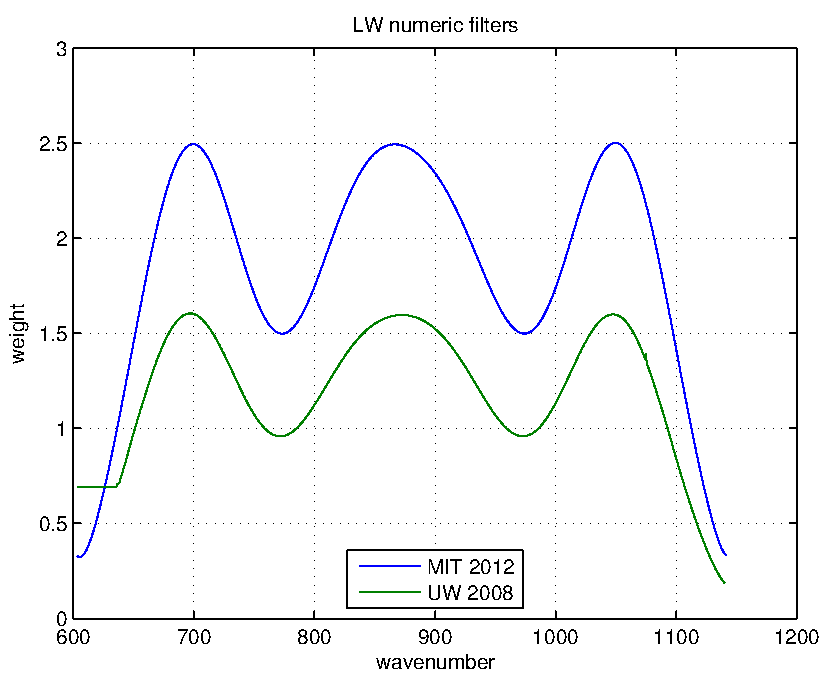
\includegraphics[scale=0.6]{figures/filters_LW.pdf}
\end{center}

LW filters from UW 2008 frequency domain and MIT 2012 time domain
representations

\end{frame}
%----------- slide --------------------------------------------------%
\begin{frame}
\frametitle{MW numeric filters}

\begin{center}
  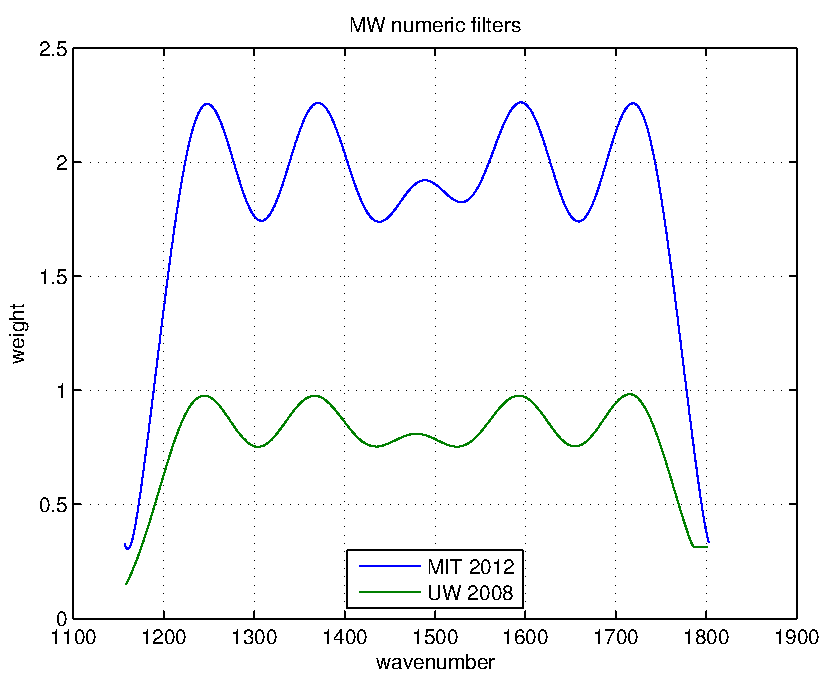
\includegraphics[scale=0.6]{figures/filters_MW.pdf}
\end{center}

MW filters from UW 2008 frequency domain and MIT 2012 time domain
representations

\end{frame}
%----------- slide --------------------------------------------------%
\begin{frame}
\frametitle{SW numeric filters}

\begin{center}
  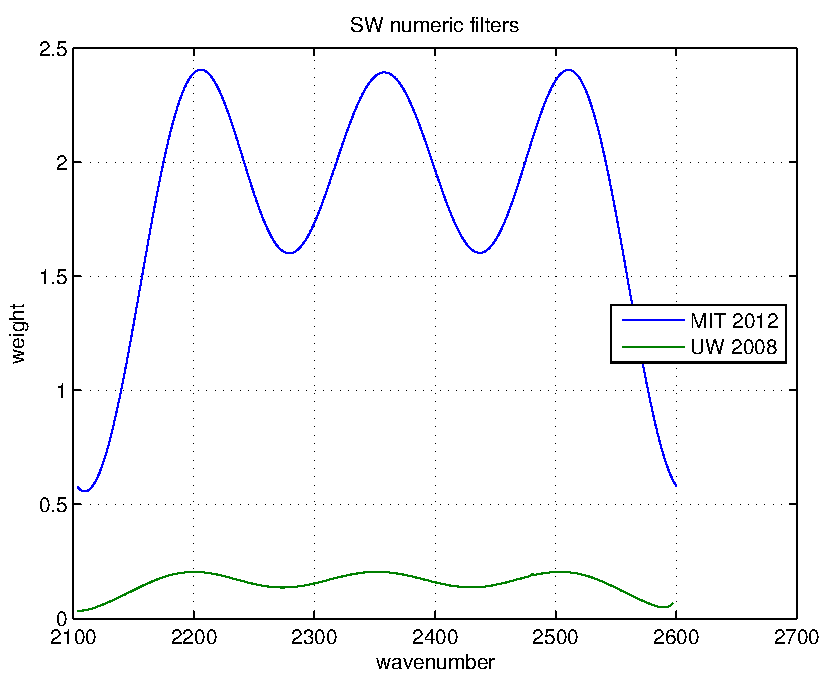
\includegraphics[scale=0.6]{figures/filters_SW.pdf}
\end{center}

SW filters from UW 2008 frequency domain and MIT 2012 time domain
representations

\end{frame}
%----------- slide --------------------------------------------------%
\end{document}

